\renewcommand{\mark}[1]{\node[circle,fill=#1] {};}
\newcommand{\emptycirc}{\node[circle,draw] {};}

\begin{frame}[<+->]{Laufzeit von \texttt{FindISG} - (1)}{}
  {\beamerblue Vor unseren Änderungen.\newline}
  \begin{figure}
    \centering
    \begin{tikzpicture}
  \matrix (m) [matrix of nodes,ampersand replacement=\&] {
\mark{black} \& \mark{black} \& \mark{black} \& \mark{black} \& \mark{black} \& \mark{black} \& \mark{black} \& \mark{black} \& \mark{black} \& \mark{black}\\
\mark{black} \& \mark{black} \& \mark{black} \& \mark{black} \& \mark{black} \& \mark{black} \& \mark{black} \& \mark{black} \& \mark{black} \& \mark{black}\\
\mark{black} \& \mark{black} \& \mark{black} \& \mark{black} \& \mark{black} \& \mark{black} \& \mark{black} \& \mark{black} \& \mark{black} \& \mark{black}\\
\mark{black} \& \mark{black} \& \mark{black} \& \mark{black} \& \mark{black} \& \mark{black} \& \mark{black} \& \mark{black} \& \mark{black} \& \mark{black}\\
\mark{black} \& \mark{black} \& \mark{black} \& \mark{black} \& \mark{black} \& \mark{black} \& \mark{black} \& \mark{black} \& \mark{black} \& \mark{black}\\
\mark{black} \& \mark{black} \& \mark{black} \& \mark{black} \& \mark{black} \& \mark{black} \& \mark{black} \& \mark{black} \& \mark{black} \& \mark{black}\\
\mark{black} \& \mark{black} \& \mark{black} \& \mark{black} \& \mark{black} \& \mark{black} \& \mark{black} \& \mark{black} \& \mark{black} \& \mark{black}\\
\mark{black} \& \mark{black} \& \mark{black} \& \mark{black} \& \mark{black} \& \mark{black!50!white} \& \mark{black!50!white} \& \mark{black!50!white} \& \mark{black!50!white} \& \mark{black!50!white}\\
\mark{black!50!white} \& \mark{black!50!white} \& \mark{black!50!white} \& \mark{black!50!white} \& \mark{black!50!white} \& \mark{black!50!white} \& \mark{black!50!white} \& \mark{black!50!white} \& \mark{black!50!white} \& \mark{black!50!white}\\
\mark{black!50!white} \& \mark{black!50!white} \& \mark{black!50!white} \& \mark{black!50!white} \& \mark{black!50!white} \& \mark{black!50!white} \& \mark{black!50!white} \& \mark{black!50!white} \& \mark{black!50!white} \& \mark{black!50!white}\\
};
\end{tikzpicture}

  \end{figure}
  \begin{center}
    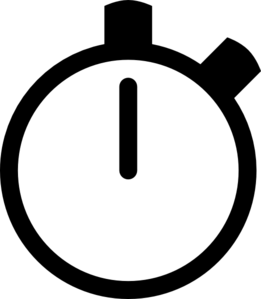
\includegraphics[width=0.4cm]{stop-watch-icon.png} \bf ~~~ 150 Minuten
  \end{center}
\end{frame}

\begin{frame}[<+->]{Laufzeit von \texttt{FindISG} - (2)}{}
  {\beamerblue Verwendung der ersten Version des Java-VF2 anstelle der C++ Version.\newline}
  \begin{figure}
    \centering
    \begin{tikzpicture}
  \matrix (m) [matrix of nodes,ampersand replacement=\&] {
    \mark{black!50!white} \& \mark{black!50!white} \& \mark{black!50!white} \& \mark{black!50!white} \& \mark{black!50!white} \& \mark{black!50!white} \& \mark{black!50!white} \& \mark{black!50!white} \& \mark{black!50!white} \& \mark{black!50!white}\\
    \mark{black!50!white} \& \mark{black!50!white} \& \mark{black!50!white} \& \mark{black!50!white} \& \mark{black!50!white} \& \mark{black!50!white} \& \mark{black!50!white} \& \mark{black!50!white} \& \mark{black!50!white} \& \mark{black!50!white}\\
    \mark{black!50!white} \& \mark{black!50!white} \& \mark{black!50!white} \& \mark{black!50!white} \& \mark{black!50!white} \& \mark{black!50!white} \& \mark{black!50!white} \& \mark{black!50!white} \& \mark{black!50!white} \& \mark{black!50!white}\\
    \mark{black!50!white} \& \mark{black!50!white} \& \mark{black!50!white} \& \mark{black!50!white} \& \mark{black!50!white} \& \mark{black!50!white} \& \mark{black!50!white} \& \mark{black!50!white} \& \mark{black!50!white} \& \mark{black!50!white}\\
    \mark{black!50!white} \& \mark{black!50!white} \& \mark{black!50!white} \& \mark{black!50!white} \& \mark{black!50!white} \& \mark{black!50!white} \& \mark{black!50!white} \& \mark{black!50!white} \& \mark{black!50!white} \& \mark{black!50!white}\\
    \mark{black!50!white} \& \mark{black!50!white} \& \mark{black!50!white} \& \mark{black!50!white} \& \mark{black!50!white} \& \mark{black!50!white} \& \mark{black!50!white} \& \mark{black!50!white} \& \mark{black!50!white} \& \mark{black!50!white}\\
    \mark{black!50!white} \& \mark{black!50!white} \& \mark{black!50!white} \& \mark{black!50!white} \& \mark{black!50!white} \& \mark{black!50!white} \& \mark{black!50!white} \& \mark{black!50!white} \& \mark{black!50!white} \& \mark{black!50!white}\\
    \mark{black!50!white} \& \mark{black!50!white} \& \mark{black!50!white} \& \mark{black!50!white} \& \mark{black!50!white} \& \mark{black!50!white} \& \mark{black!50!white} \& \mark{black!50!white} \& \mark{black!50!white} \& \mark{black!50!white}\\
    \mark{black!50!white} \& \mark{black!50!white} \& \mark{black!50!white} \& \mark{black!50!white} \& \mark{black!50!white} \& \mark{black!50!white} \& \mark{black!50!white} \& \mark{black!50!white} \& \mark{black!50!white} \& \mark{black!50!white}\\
    \mark{black!50!white} \& \mark{black!50!white} \& \mark{black!50!white} \& \mark{black!50!white} \& \mark{black!50!white} \& \mark{black!50!white} \& \mark{black!50!white} \& \mark{black!50!white} \& \mark{black!50!white} \& \mark{black!50!white}\\
  };
  \node {\textcolor{red}{\Huge \(\infty\)}};
\end{tikzpicture}

  \end{figure}
  \begin{center}
    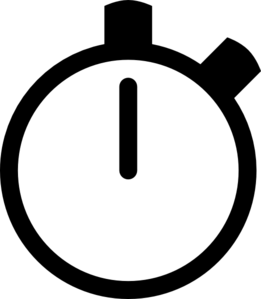
\includegraphics[width=0.4cm]{stop-watch-icon.png} \bf ~~~ über 12 Stunden
  \end{center}
\end{frame}

\begin{frame}[<+->]{Laufzeit von \texttt{FindISG} - (3)}{}
  {\beamerblue Weglassen der Erzeugung sämtlicher Subgraphen, stattdessen direkter Test
   auf Subisomorphie.}
  \begin{figure}
    \centering
    \begin{tikzpicture}
  \matrix (m) [matrix of nodes,ampersand replacement=\&] {
\mark{black} \& \mark{black} \& \mark{black} \& \mark{black} \& \mark{black} \& \mark{black} \& \mark{black} \& \mark{black} \& \mark{black} \& \mark{black}\\
\mark{black} \& \mark{black} \& \mark{black} \& \mark{black} \& \mark{black} \& \mark{black} \& \mark{black} \& \mark{black} \& \mark{black} \& \mark{black}\\
\mark{black} \& \mark{black} \& \mark{black} \& \mark{black} \& \mark{black} \& \mark{black} \& \mark{black} \& \mark{black} \& \mark{black} \& \mark{black}\\
\mark{black} \& \mark{black} \& \mark{black} \& \mark{black} \& \mark{black} \& \mark{black} \& \mark{black} \& \mark{black} \& \mark{black} \& \mark{black}\\
\mark{black} \& \mark{black} \& \mark{black} \& \mark{black} \& \mark{black} \& \mark{black} \& \mark{black} \& \mark{black} \& \mark{black} \& \mark{black}\\
\mark{black} \& \mark{black} \& \mark{black} \& \mark{black} \& \mark{black} \& \mark{black} \& \mark{black} \& \mark{black} \& \mark{black} \& \mark{black}\\
\mark{black} \& \mark{black} \& \mark{black} \& \mark{black} \& \mark{black} \& \mark{black} \& \mark{black} \& \mark{black} \& \mark{black} \& \mark{black}\\
\mark{black} \& \mark{black} \& \mark{black} \& \mark{black} \& \mark{black} \& \mark{red} \& \mark{red} \& \mark{red} \& \mark{red} \& \mark{red}\\
\mark{red} \& \mark{red} \& \mark{red} \& \mark{red} \& \mark{red} \& \mark{red} \& \mark{red} \& \mark{red} \& \mark{red} \& \mark{red}\\
\mark{red} \& \mark{red} \& \mark{red} \& \mark{red} \& \mark{red} \& \mark{red} \& \mark{red} \& \mark{red} \& \mark{red} \& \mark{red}\\
};
\end{tikzpicture}

  \end{figure}
  \begin{center}
    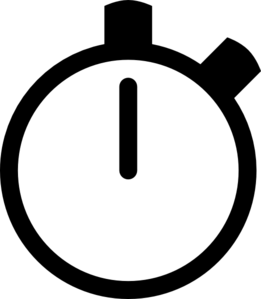
\includegraphics[width=0.4cm]{stop-watch-icon.png} \bf ~~~ 200 Minuten
  \end{center}
\end{frame}

\begin{frame}[<+->]{Laufzeit von \texttt{FindISG} - (4)}{}
  {\beamerblue Konsequente Verwendung von \texttt{VF2} in allen Isomorphietests,
   \texttt{VF2} sortiert zudem nach Knotengrad vor.}
  \begin{figure}
    \centering
    \begin{tikzpicture}
  \matrix (m) [matrix of nodes,ampersand replacement=\&] {
\mark{black} \& \mark{black} \& \mark{black} \& \mark{black} \& \mark{black} \& \mark{black} \& \mark{black} \& \mark{black} \& \mark{black} \& \mark{black}\\
\mark{black} \& \mark{black} \& \mark{black} \& \mark{black} \& \mark{black} \& \mark{black} \& \mark{black} \& \mark{black} \& \mark{black} \& \mark{black}\\
\mark{black} \& \mark{black} \& \mark{black} \& \mark{black} \& \mark{black} \& \mark{black} \& \mark{black} \& \mark{black} \& \mark{black} \& \mark{black}\\
\mark{black} \& \mark{black} \& \mark{black} \& \mark{black} \& \mark{black} \& \mark{black} \& \mark{black} \& \mark{black} \& \mark{black} \& \mark{black}\\
\mark{black} \& \mark{black} \& \mark{black} \& \mark{black} \& \mark{black} \& \mark{black} \& \mark{black} \& \mark{black} \& \mark{black} \& \mark{black}\\
\mark{black} \& \mark{black} \& \mark{black} \& \mark{black} \& \mark{black} \& \mark{black} \& \mark{black} \& \mark{black} \& \mark{black} \& \mark{black}\\
\mark{black} \& \mark{black} \& \mark{black} \& \mark{black} \& \mark{black} \& \mark{black} \& \mark{black} \& \mark{black} \& \mark{black} \& \mark{black}\\
\mark{black} \& \mark{black} \& \mark{black} \& \mark{black} \& \mark{black} \& \emptycirc \& \emptycirc \& \emptycirc \& \emptycirc \& \emptycirc\\
\emptycirc \& \emptycirc \& \emptycirc \& \emptycirc \& \emptycirc \& \emptycirc \& \emptycirc \& \emptycirc \& \emptycirc \& \emptycirc\\
\emptycirc \& \emptycirc \& \emptycirc \& \emptycirc \& \emptycirc \& \emptycirc \& \emptycirc \& \emptycirc \& \emptycirc \& \emptycirc\\
};
\end{tikzpicture}

  \end{figure}
  \begin{center}
    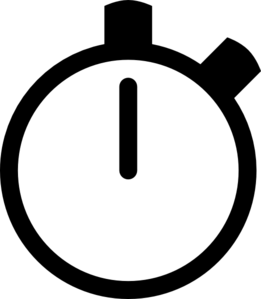
\includegraphics[width=0.4cm]{stop-watch-icon.png} \bf ~~~ wieder 150 Minuten
  \end{center}
\end{frame}

\begin{frame}[<+->]{Laufzeit von \texttt{FindISG} - (5)}{}
  {\beamerblue Parallelisierung der Subisomorphieberechnung für große Graphen.\newline}
  \begin{figure}
    \centering
    \begin{tikzpicture}
  \matrix (m) [matrix of nodes,ampersand replacement=\&] {
\mark{black} \& \mark{black} \& \mark{black} \& \mark{black} \& \mark{black} \& \mark{black} \& \mark{black} \& \mark{black} \& \mark{black} \& \mark{black}\\
\mark{black} \& \mark{black} \& \mark{black} \& \mark{black} \& \mark{black} \& \mark{black} \& \mark{black} \& \mark{black} \& \mark{black} \& \mark{black}\\
\mark{black} \& \mark{black} \& \mark{black} \& \mark{black} \& \mark{black} \& \emptycirc \& \emptycirc \& \emptycirc \& \emptycirc \& \emptycirc\\
\emptycirc \& \emptycirc \& \emptycirc \& \emptycirc \& \emptycirc \& \emptycirc \& \emptycirc \& \emptycirc \& \emptycirc \& \emptycirc\\
\emptycirc \& \emptycirc \& \emptycirc \& \emptycirc \& \emptycirc \& \emptycirc \& \emptycirc \& \emptycirc \& \emptycirc \& \emptycirc\\
\emptycirc \& \emptycirc \& \emptycirc \& \emptycirc \& \emptycirc \& \emptycirc \& \emptycirc \& \emptycirc \& \emptycirc \& \emptycirc\\
\emptycirc \& \emptycirc \& \emptycirc \& \emptycirc \& \emptycirc \& \emptycirc \& \emptycirc \& \emptycirc \& \emptycirc \& \emptycirc\\
\emptycirc \& \emptycirc \& \emptycirc \& \emptycirc \& \emptycirc \& \emptycirc \& \emptycirc \& \emptycirc \& \emptycirc \& \emptycirc\\
\emptycirc \& \emptycirc \& \emptycirc \& \emptycirc \& \emptycirc \& \emptycirc \& \emptycirc \& \emptycirc \& \emptycirc \& \emptycirc\\
\emptycirc \& \emptycirc \& \emptycirc \& \emptycirc \& \emptycirc \& \emptycirc \& \emptycirc \& \emptycirc \& \emptycirc \& \emptycirc\\
};
\end{tikzpicture}

  \end{figure}
  \begin{center}
    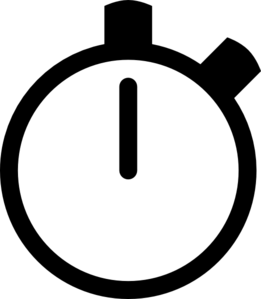
\includegraphics[width=0.4cm]{stop-watch-icon.png} \bf ~~~ 50 Minuten
  \end{center}
\end{frame}

\begin{frame}[<+->]{Laufzeit von \texttt{FindISG} - (6)}{}
  {\beamerblue Caching von Kanten im \texttt{VF2}.\newline}
  \begin{figure}
    \centering
    \begin{tikzpicture}
  \matrix (m) [matrix of nodes,ampersand replacement=\&] {
\mark{black} \& \mark{black} \& \mark{black} \& \mark{black} \& \mark{black} \& \mark{black} \& \mark{black} \& \mark{black} \& \mark{black} \& \mark{black}\\
\mark{black} \& \mark{black} \& \mark{black} \& \mark{black} \& \mark{black} \& \emptycirc \& \emptycirc \& \emptycirc \& \emptycirc \& \emptycirc\\
\emptycirc \& \emptycirc \& \emptycirc \& \emptycirc \& \emptycirc \& \emptycirc \& \emptycirc \& \emptycirc \& \emptycirc \& \emptycirc\\
\emptycirc \& \emptycirc \& \emptycirc \& \emptycirc \& \emptycirc \& \emptycirc \& \emptycirc \& \emptycirc \& \emptycirc \& \emptycirc\\
\emptycirc \& \emptycirc \& \emptycirc \& \emptycirc \& \emptycirc \& \emptycirc \& \emptycirc \& \emptycirc \& \emptycirc \& \emptycirc\\
\emptycirc \& \emptycirc \& \emptycirc \& \emptycirc \& \emptycirc \& \emptycirc \& \emptycirc \& \emptycirc \& \emptycirc \& \emptycirc\\
\emptycirc \& \emptycirc \& \emptycirc \& \emptycirc \& \emptycirc \& \emptycirc \& \emptycirc \& \emptycirc \& \emptycirc \& \emptycirc\\
\emptycirc \& \emptycirc \& \emptycirc \& \emptycirc \& \emptycirc \& \emptycirc \& \emptycirc \& \emptycirc \& \emptycirc \& \emptycirc\\
\emptycirc \& \emptycirc \& \emptycirc \& \emptycirc \& \emptycirc \& \emptycirc \& \emptycirc \& \emptycirc \& \emptycirc \& \emptycirc\\
\emptycirc \& \emptycirc \& \emptycirc \& \emptycirc \& \emptycirc \& \emptycirc \& \emptycirc \& \emptycirc \& \emptycirc \& \emptycirc\\
};
\end{tikzpicture}

  \end{figure}
  \begin{center}
    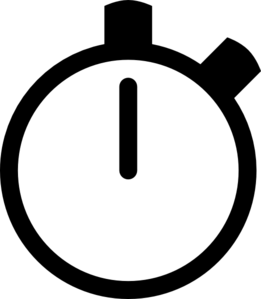
\includegraphics[width=0.4cm]{stop-watch-icon.png} \bf ~~~ 30 Minuten
  \end{center}
\end{frame}

\begin{frame}[<+->]{Laufzeit von \texttt{FindISG} - (7)}{}
  {\beamerblue Isomorphietest auf dem Graphen bzw. Komplement mit weniger Kanten.\newline}
  \begin{figure}
    \centering
    \begin{tikzpicture}
  \matrix (m) [matrix of nodes,ampersand replacement=\&] {
\mark{black} \& \mark{black} \& \mark{black} \& \mark{black} \& \mark{black} \& \mark{black} \& \emptycirc \& \emptycirc \& \emptycirc \& \emptycirc\\
\emptycirc \& \emptycirc \& \emptycirc \& \emptycirc \& \emptycirc \& \emptycirc \& \emptycirc \& \emptycirc \& \emptycirc \& \emptycirc\\
\emptycirc \& \emptycirc \& \emptycirc \& \emptycirc \& \emptycirc \& \emptycirc \& \emptycirc \& \emptycirc \& \emptycirc \& \emptycirc\\
\emptycirc \& \emptycirc \& \emptycirc \& \emptycirc \& \emptycirc \& \emptycirc \& \emptycirc \& \emptycirc \& \emptycirc \& \emptycirc\\
\emptycirc \& \emptycirc \& \emptycirc \& \emptycirc \& \emptycirc \& \emptycirc \& \emptycirc \& \emptycirc \& \emptycirc \& \emptycirc\\
\emptycirc \& \emptycirc \& \emptycirc \& \emptycirc \& \emptycirc \& \emptycirc \& \emptycirc \& \emptycirc \& \emptycirc \& \emptycirc\\
\emptycirc \& \emptycirc \& \emptycirc \& \emptycirc \& \emptycirc \& \emptycirc \& \emptycirc \& \emptycirc \& \emptycirc \& \emptycirc\\
\emptycirc \& \emptycirc \& \emptycirc \& \emptycirc \& \emptycirc \& \emptycirc \& \emptycirc \& \emptycirc \& \emptycirc \& \emptycirc\\
\emptycirc \& \emptycirc \& \emptycirc \& \emptycirc \& \emptycirc \& \emptycirc \& \emptycirc \& \emptycirc \& \emptycirc \& \emptycirc\\
\emptycirc \& \emptycirc \& \emptycirc \& \emptycirc \& \emptycirc \& \emptycirc \& \emptycirc \& \emptycirc \& \emptycirc \& \emptycirc\\
};
\end{tikzpicture}

  \end{figure}
  \begin{center}
    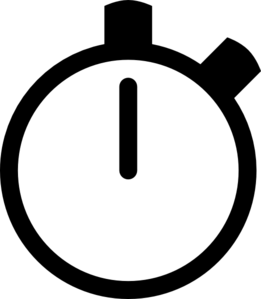
\includegraphics[width=0.4cm]{stop-watch-icon.png} \bf ~~~ 12 Minuten
  \end{center}
\end{frame}

\begin{frame}[<+->]{Laufzeit von \texttt{FindISG} - (8)}{}
  {\beamerblue Weiterentwicklung des \texttt{VF2}...\newline}
  \begin{figure}
    \centering
    \begin{tikzpicture}
  \matrix (m) [matrix of nodes,ampersand replacement=\&] {
\mark{black} \& \mark{black} \& \emptycirc \& \emptycirc \& \emptycirc \& \emptycirc \& \emptycirc \& \emptycirc \& \emptycirc \& \emptycirc\\
\emptycirc \& \emptycirc \& \emptycirc \& \emptycirc \& \emptycirc \& \emptycirc \& \emptycirc \& \emptycirc \& \emptycirc \& \emptycirc\\
\emptycirc \& \emptycirc \& \emptycirc \& \emptycirc \& \emptycirc \& \emptycirc \& \emptycirc \& \emptycirc \& \emptycirc \& \emptycirc\\
\emptycirc \& \emptycirc \& \emptycirc \& \emptycirc \& \emptycirc \& \emptycirc \& \emptycirc \& \emptycirc \& \emptycirc \& \emptycirc\\
\emptycirc \& \emptycirc \& \emptycirc \& \emptycirc \& \emptycirc \& \emptycirc \& \emptycirc \& \emptycirc \& \emptycirc \& \emptycirc\\
\emptycirc \& \emptycirc \& \emptycirc \& \emptycirc \& \emptycirc \& \emptycirc \& \emptycirc \& \emptycirc \& \emptycirc \& \emptycirc\\
\emptycirc \& \emptycirc \& \emptycirc \& \emptycirc \& \emptycirc \& \emptycirc \& \emptycirc \& \emptycirc \& \emptycirc \& \emptycirc\\
\emptycirc \& \emptycirc \& \emptycirc \& \emptycirc \& \emptycirc \& \emptycirc \& \emptycirc \& \emptycirc \& \emptycirc \& \emptycirc\\
\emptycirc \& \emptycirc \& \emptycirc \& \emptycirc \& \emptycirc \& \emptycirc \& \emptycirc \& \emptycirc \& \emptycirc \& \emptycirc\\
\emptycirc \& \emptycirc \& \emptycirc \& \emptycirc \& \emptycirc \& \emptycirc \& \emptycirc \& \emptycirc \& \emptycirc \& \emptycirc\\
};
\end{tikzpicture}

  \end{figure}
  \begin{center}
    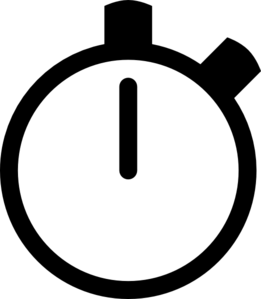
\includegraphics[width=0.4cm]{stop-watch-icon.png} \bf ~~~ 4 Minuten
  \end{center}
\end{frame}

\begin{frame}[<+->]{Laufzeit von \texttt{FindISG} - (9)}{}
  {\beamerblue ...\texttt{VF2} nochmals verbessert.\newline}
  \begin{figure}
    \centering
    \begin{tikzpicture}
  \matrix (m) [matrix of nodes,ampersand replacement=\&] {
\mark{black} \& \emptycirc \& \emptycirc \& \emptycirc \& \emptycirc \& \emptycirc \& \emptycirc \& \emptycirc \& \emptycirc \& \emptycirc\\
\emptycirc \& \emptycirc \& \emptycirc \& \emptycirc \& \emptycirc \& \emptycirc \& \emptycirc \& \emptycirc \& \emptycirc \& \emptycirc\\
\emptycirc \& \emptycirc \& \emptycirc \& \emptycirc \& \emptycirc \& \emptycirc \& \emptycirc \& \emptycirc \& \emptycirc \& \emptycirc\\
\emptycirc \& \emptycirc \& \emptycirc \& \emptycirc \& \emptycirc \& \emptycirc \& \emptycirc \& \emptycirc \& \emptycirc \& \emptycirc\\
\emptycirc \& \emptycirc \& \emptycirc \& \emptycirc \& \emptycirc \& \emptycirc \& \emptycirc \& \emptycirc \& \emptycirc \& \emptycirc\\
\emptycirc \& \emptycirc \& \emptycirc \& \emptycirc \& \emptycirc \& \emptycirc \& \emptycirc \& \emptycirc \& \emptycirc \& \emptycirc\\
\emptycirc \& \emptycirc \& \emptycirc \& \emptycirc \& \emptycirc \& \emptycirc \& \emptycirc \& \emptycirc \& \emptycirc \& \emptycirc\\
\emptycirc \& \emptycirc \& \emptycirc \& \emptycirc \& \emptycirc \& \emptycirc \& \emptycirc \& \emptycirc \& \emptycirc \& \emptycirc\\
\emptycirc \& \emptycirc \& \emptycirc \& \emptycirc \& \emptycirc \& \emptycirc \& \emptycirc \& \emptycirc \& \emptycirc \& \emptycirc\\
\emptycirc \& \emptycirc \& \emptycirc \& \emptycirc \& \emptycirc \& \emptycirc \& \emptycirc \& \emptycirc \& \emptycirc \& \emptycirc\\
};
\end{tikzpicture}

  \end{figure}
  \begin{center}
    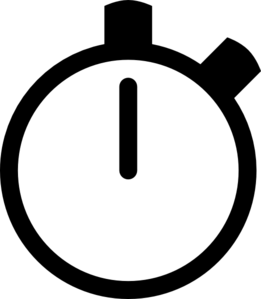
\includegraphics[width=0.4cm]{stop-watch-icon.png} \bf ~~~ 2 Minuten
  \end{center}
\end{frame}

\begin{frame}[<+->]{\texttt{FindISG} - Resultat}{}
  \begin{columns}<.->
    \column{0.5\textwidth}<.->
      \begin{figure}
        \centering
        \begin{tikzpicture}
  \matrix (m) [matrix of nodes,ampersand replacement=\&] {
\mark{black} \& \mark{black} \& \mark{black} \& \mark{black} \& \mark{black} \& \mark{black} \& \mark{black} \& \mark{black} \& \mark{black} \& \mark{black}\\
\mark{black} \& \mark{black} \& \mark{black} \& \mark{black} \& \mark{black} \& \mark{black} \& \mark{black} \& \mark{black} \& \mark{black} \& \mark{black}\\
\mark{black} \& \mark{black} \& \mark{black} \& \mark{black} \& \mark{black} \& \mark{black} \& \mark{black} \& \mark{black} \& \mark{black} \& \mark{black}\\
\mark{black} \& \mark{black} \& \mark{black} \& \mark{black} \& \mark{black} \& \mark{black} \& \mark{black} \& \mark{black} \& \mark{black} \& \mark{black}\\
\mark{black} \& \mark{black} \& \mark{black} \& \mark{black} \& \mark{black} \& \mark{black} \& \mark{black} \& \mark{black} \& \mark{black} \& \mark{black}\\
\mark{black} \& \mark{black} \& \mark{black} \& \mark{black} \& \mark{black} \& \mark{black} \& \mark{black} \& \mark{black} \& \mark{black} \& \mark{black}\\
\mark{black} \& \mark{black} \& \mark{black} \& \mark{black} \& \mark{black} \& \mark{black} \& \mark{black} \& \mark{black} \& \mark{black} \& \mark{black}\\
\mark{black} \& \mark{black} \& \mark{black} \& \mark{black} \& \mark{black} \& \mark{black!50!white} \& \mark{black!50!white} \& \mark{black!50!white} \& \mark{black!50!white} \& \mark{black!50!white}\\
\mark{black!50!white} \& \mark{black!50!white} \& \mark{black!50!white} \& \mark{black!50!white} \& \mark{black!50!white} \& \mark{black!50!white} \& \mark{black!50!white} \& \mark{black!50!white} \& \mark{black!50!white} \& \mark{black!50!white}\\
\mark{black!50!white} \& \mark{black!50!white} \& \mark{black!50!white} \& \mark{black!50!white} \& \mark{black!50!white} \& \mark{black!50!white} \& \mark{black!50!white} \& \mark{black!50!white} \& \mark{black!50!white} \& \mark{black!50!white}\\
};
\end{tikzpicture}

      \end{figure}
    \column{0.5\textwidth}<.->
      \begin{figure}
        \centering
        \begin{tikzpicture}
  \matrix (m) [matrix of nodes,ampersand replacement=\&] {
\mark{black} \& \emptycirc \& \emptycirc \& \emptycirc \& \emptycirc \& \emptycirc \& \emptycirc \& \emptycirc \& \emptycirc \& \emptycirc\\
\emptycirc \& \emptycirc \& \emptycirc \& \emptycirc \& \emptycirc \& \emptycirc \& \emptycirc \& \emptycirc \& \emptycirc \& \emptycirc\\
\emptycirc \& \emptycirc \& \emptycirc \& \emptycirc \& \emptycirc \& \emptycirc \& \emptycirc \& \emptycirc \& \emptycirc \& \emptycirc\\
\emptycirc \& \emptycirc \& \emptycirc \& \emptycirc \& \emptycirc \& \emptycirc \& \emptycirc \& \emptycirc \& \emptycirc \& \emptycirc\\
\emptycirc \& \emptycirc \& \emptycirc \& \emptycirc \& \emptycirc \& \emptycirc \& \emptycirc \& \emptycirc \& \emptycirc \& \emptycirc\\
\emptycirc \& \emptycirc \& \emptycirc \& \emptycirc \& \emptycirc \& \emptycirc \& \emptycirc \& \emptycirc \& \emptycirc \& \emptycirc\\
\emptycirc \& \emptycirc \& \emptycirc \& \emptycirc \& \emptycirc \& \emptycirc \& \emptycirc \& \emptycirc \& \emptycirc \& \emptycirc\\
\emptycirc \& \emptycirc \& \emptycirc \& \emptycirc \& \emptycirc \& \emptycirc \& \emptycirc \& \emptycirc \& \emptycirc \& \emptycirc\\
\emptycirc \& \emptycirc \& \emptycirc \& \emptycirc \& \emptycirc \& \emptycirc \& \emptycirc \& \emptycirc \& \emptycirc \& \emptycirc\\
\emptycirc \& \emptycirc \& \emptycirc \& \emptycirc \& \emptycirc \& \emptycirc \& \emptycirc \& \emptycirc \& \emptycirc \& \emptycirc\\
};
\end{tikzpicture}

      \end{figure}
  \end{columns}
  \begin{center}
    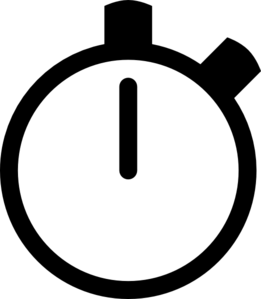
\includegraphics[width=0.4cm]{stop-watch-icon.png} \bf ~~~ Von 150 Minuten auf 2 Minuten
  \end{center}
\end{frame}
